\documentclass[Main.tex]{subfiles}

\begin{document}
\section{Non-Spatial Model Applications}
This section provides a brief run-down of some well studied swarm robot applications and the important results ascertained from them. While this list is by no means a comprehensive evaluation of every single swarm robot algorithm ever developed, the featured algorithms share a development model similar to the one described in the previous section, consisting of a PFSM and the ODE (or Difference Equation, DE) system that defines their macroscopic behavior. The final model described in this section is based on our ongoing research work on multi-robot coordination using a response threshold function.


% 1 ============================================================================
\subsection{Object Clustering}
Object clustering, or aggregation, is one of the early applications for robot swarms inspired from transport techniques seen in ant colonies. It was introduced in~\cite{Martinoli1995} as an example of collective, non-cooperative behavior. The task involves moving objects that have been scattered over a region and collecting them in a pile without explicit communication or global positioning. It is an example of non-cooperative behavior since every agent is capable of moving objects on its own and thus no cooperation is required between individuals to successfully complete the task.

Agassounon, Kalra and Martinoli introduce worker allocation via threshold functions as a variant to the original object clustering experiment in~\cite{Kalra2006, Agassounon2001} and expand the results in~\cite{Agassounon2002a}. Here, agents decide whether or not to help with the global task (stick collecting) based on their local perception of the degree of completion of the task. While earlier attempts at threshold based collective algorithms for robots suffer from scalability issues arising from explicit communication~\cite{Parker1998} between agents or the need for a centralized supervisor~\cite{Krieger2000}, the collaborative approach presented in~\cite{Agassounon2001} employs a wholly distributed strategy where agents use only local observations to make work vs. rest decisions. 

\begin{figure}[!htb]
\centering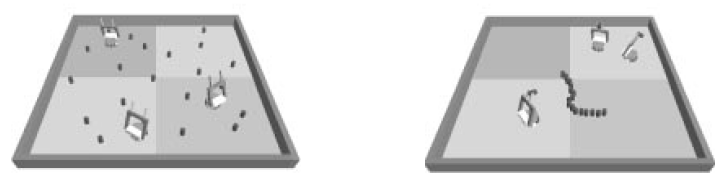
\includegraphics[width=\textwidth]{martinoliMondadaStickCollect.png}
\caption{Webots simulation of Khepera robots performing object clustering. Left image shows the initial placement of robots/sticks in the arena while the right image shows the successful completion of the task.}\label{fig:stickforage}
\end{figure}


\subsubsection*{Results}
\begin{figure}[!htb]
\centering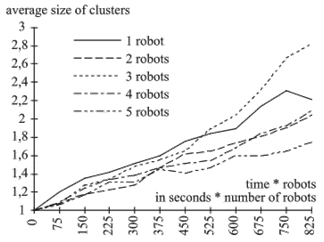
\includegraphics[width=.5\textwidth]{clusterRes.png}
\caption{Results from the original object clustering task without threshold based worker allocation emphasizing the non-cooperative nature of the task, i.e. more robots do not necessarily complete the task faster.}\label{fig:clusterres}
\end{figure}

It is shown via physical experiments in~\cite{Martinoli1995} that adding agents to the task only speeds up the rate of collection to a certain threshold, and that overall efficiency is not necessarily maximized by adding more agents (as seen in Figure~\ref{fig:clusterres}).

For the sake of brevity, results from the threshold based worker allocation variant of this experiment have been excluded from this discussion but can be found in~\cite{Agassounon2001, Agassounon2002a, agassounon2004}.


% 2 ============================================================================
\subsection{The Stick Pulling Experiment}\label{sec:stickpull}

\begin{figure}[!htb]
\centering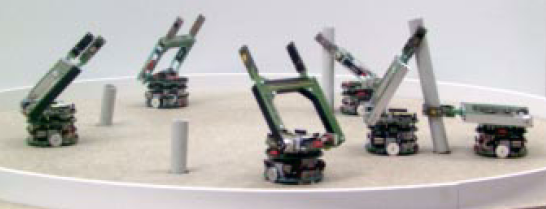
\includegraphics[width=.8\textwidth]{stickpullPhysical.png}
\caption{A real experimental setup for the 2-robot stick pulling experiment showing a team of two robots successfully pulling a stick out of the ground.}\label{fig:stickpull}
\end{figure}

Introduced alongside object clustering in~\cite{Martinoli1995}---later extended and studied in further detail~\cite{Martinoli1999, Martinoli1999a, Ijspeert2001, Lerman2001, Martinoli2004}---the aim of this experiment is to pull long sticks out of the ground using pairs of collaborating robots. Each stick is placed deep enough into the floor that a single robot cannot successfully pull it out. Therefore, the agent's goal is to first find a stick and then either wait at that stick if another robot is not already at it, or to help the robot currently at the stick. 

The robots have an internal timer that begins to tick down as they wait at a stick. This parameter is referred to as the \emph{gripping time} or \emph{wait time} in the experiment. If a fellow robot does not come to help before the gripping time expires then the robot lets go of the stick it is currently at and tries to find another stick. Adjusting the gripping time for each agent non-trivially affects the overall outcome the collaborative task. Once a stick is successfully pulled out of the ground by a coalition of two robots, they perform a \emph{success dance} and then break their coalition. Each robot then returns to the search state. 

Sticks that are pulled out of the ground are replaced by a human so that the total number of sticks to pull does not change during the course of the experiment. Likewise, the number of agents is constant over course of the experiment. The goal of the experiment is to maximize the rate of collaboration between robots or, in other words, maximize the number of sticks being pulled out of the ground per unit time.

The robots used for this task are called \emph{Khepera} robots. The technical specification of the robot are given in Table~\ref{tab:khepera}. The only modification made to the original hardware design for this experiment is that each robot is outfitted with a single-joint gripper arm so that it can grip and lift sticks, as seen in Figure~\ref{fig:khepbot}.

\begin{figure}[!htb]
\centering 
\begin{subfigure}[b]{6.5cm}
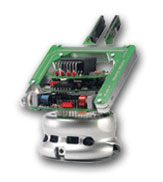
\includegraphics[width=5cm]{khepera2robot.png}
\centering\caption{The Khepera-II robot used in the \emph{Stick Pulling Experiment} by Martinoli et. al.}\label{fig:khepbot}
\end{subfigure}
\qquad\centering
\begin{subfigure}[b]{6.5cm}
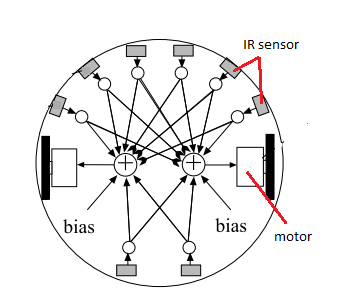
\includegraphics[width=5cm]{kheperascem.png}
\centering\caption{Neural net that controls sensory feedback on the Khepera-II robot for the stick pulling experiment.}\label{fig:khepschem}
\end{subfigure}
\caption{}\label{fig:kheperastick}
\end{figure}

\rowcolors{1}{lightgray}{white}
\begin{table}[htb]
\centering\begin{tabular}{|*{4}{c|}}
\hline
Diameter & Height & Mass & Velocity \\
$55$mm & $30$mm & $80$g & $0.02$ to $1.0$ms$^{-1}$ \\ \hline
Battery Life & CPU & RAM & EEPROM \\
45min & Motorola 68331 @ $16$MHz & $256$KB & $512$KB \\ \hline
OS & Motors & \multicolumn{2}{c|}{Sensors}\\
$\mu$KOS (RTOS) & 2 DC brushed servos & \multicolumn{2}{c|}{8 IR proximity and ambient light}\\
\hline
\end{tabular}
\caption{Hardware specifications of the Khepera-II robots used in the object clustering and stick pulling experiments.}\label{tab:khepera}
\end{table}
\rowcolors{1}{white}{white}


\subsubsection*{Results}
A particularly interesting insight derived from the classical stick pulling experiment and studied further in~\cite{Ijspeert2001} is the problem of wait-time parameter optimization. As mentioned earlier, in section~\ref{sec:opt}, parameter discovery and optimization are recurring tasks associated with modeling swarm systems. The sick pulling experiment provides a good practical experiment where optimization of swarm systems can be studied---the important system parameter being gripping-time of the agents.

It is found that for the case where two robots are needed to pull out a stick, an optimum wait-time exists for maximizing the rate of sticks pulled when the number of robots is less than or equal to the number of sticks in the arena (see Figure~\ref{fig:stickopt}). Intuitively, if we have more robots than sticks, the best strategy for a robot at a stick is to just wait forever since there will be at least one robot still searching at all times. On the other hand, if there are fewer (or equal) robots than sticks, the strategy of waiting forever could cause a deadlock situation in the arena where every robot is at an individual stick waiting for a partner to arrive.

\begin{figure}[!ht]
\centering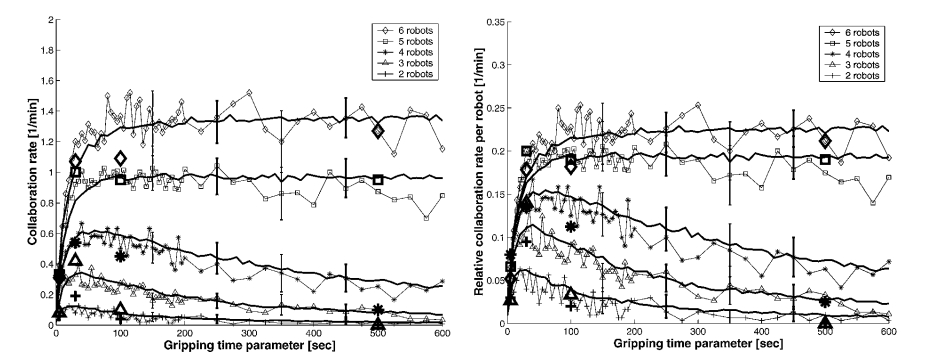
\includegraphics[width=.85\textwidth]{stickopt.png}
\centering\caption{Left: Collaboration rate as a function of the gripping time in homogeneous groups of robots. The large single markers correspond to the results with the real robots, the linked small markers to those with the Webots simulator, and the underlying continuous lines to those with the probabilistic simulation. Right: Relative collaboration rate per robot (i.e., the average number of collaborations over time to which one robot participates by either making a first or second grip). Error-bars correspond to $\pm$ standard deviations of the results with the probabilistic model (thicker bars) and with Webot (thin lines). For reasons of clarity, only some errorbars are shown and results are only shown for gripping time parameters up to 600s.}\label{fig:stickopt}
\end{figure}


% 3 ============================================================================
\subsection{Coalition Formation}
\begin{figure}[!ht]
\centering\begin{subfigure}{.5\textwidth}
\centering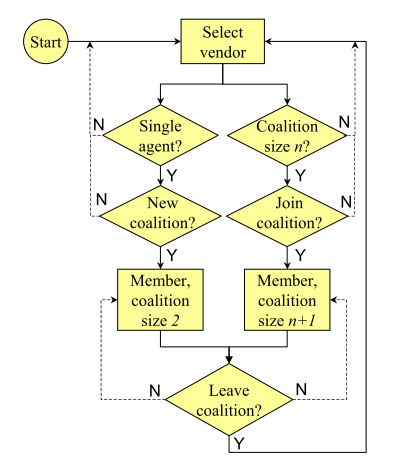
\includegraphics[width=6cm]{coalflowchart.png}
\caption{}\label{fig:coalfl}
\end{subfigure}~
\centering\begin{subfigure}{.5\textwidth}
\centering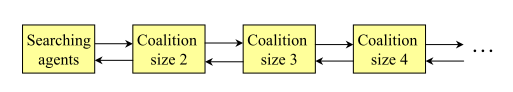
\includegraphics[width=6cm]{coalfsm.png}
\caption{}\label{fig:coalfsm}
\end{subfigure}
\caption{The flowchart and associated FSM used to describe the robot controller for coalition formation experiments are discussed by Lerman et al.}\label{fig:coal}
\end{figure}

A practical swarm optimization strategy for e-commerce applications was introduced by Lerman et al. in~\cite{Lerman2000, Lerman2001a, Lerman2001b}. Given a set of sellers for a specific product, the goal of the agent (or buyer) is to minimize cost per unit by forming coalitions with other buyers to get group discounts. 

A coalition between two or more buyers is formed if they are all purchasing the same product from the same seller. Agents are free to join or leave a coalition on their own accord but entire coalitions are not allowed to switch sellers. Discounts given to buyers are directly proportional to the size of the buying coalition. Due to storage or other constraints, sellers only keep a certain amount of the product for sale which, in turn, restricts coalition sizes. A product is kept on sale for a pre-determined period of time buy a seller after which all transactions are completed and the product is taken off the market. The flowchart and FSM for the process described above is seen in Figure~\ref{fig:coal}.

\subsubsection*{Results}
This application has been mainly used to illustrate the use of differential equation, macro-level models for studying multi-agent systems\cite{Lerman2001a, Lerman2001b}. The analysis provided explains how even a ``greedy'' agent based approach can lead to maximal utility gains for the entire system. This is a recurring property of many swarm systems---decisions are often made by an individual agent based only on local information but the effect of the decision is felt globally throughout the system.

\begin{figure}[!ht]
\centering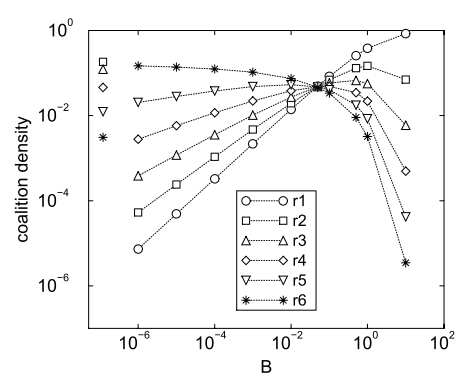
\includegraphics[width=.5\textwidth]{coalDensity.png}
\caption{Plot showing utility gain in the coalition experiment with group sizes ranging from 1 to 6 per coalition and varying attachment/detachment rates}\label{fig:coaldensity}
\end{figure}

Figure~\ref{fig:coaldensity} above shows the results obtained from solving the macro-level equations associated with this experiment for coalition sizes of 1--6 robots. Discussion of this graph in~\cite{Lerman2000} suggests that there is only a small utility gain in the case where agents are allowed to form coalitions but not leave them. However, there is a very large utility gain in the case where agents can both, form and leave coalitions at will. The caveat is that attachment and detachment rate must be kept very low. For large detachment rates, there is again virtually no utility gain, as the system is composed mainly of unaffiliated agents.

Utility gain is a measure of profit per agent computed by,
\begin{equation*}
G = Np - \sum\limits_{n=1}^{m}p_n nr_n
\end{equation*}
where $N$ is the total number of agents, $p_n$ is the coalition price dependent on the coalition size ($p_n = p - \Delta p(n - 1)$, $\Delta p =$ price decrement, $p =$ base price), and $r_n$ is the number of coalitions of size $n$. 

% 4 ============================================================================
\subsection{Cockroach Aggregation}
\begin{figure}[!htb]
\centering\begin{subfigure}{.5\textwidth}
\centering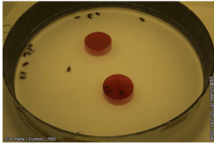
\includegraphics[width=6cm]{cockroachagg.png}
\caption{A snapshot of the real cockroach aggregation experiment conducted by Jeanson et al. The cockroaches cluster under red protective covers that block light.}\label{fig:roachagg}
\end{subfigure}~
\centering\begin{subfigure}{.5\textwidth}
\centering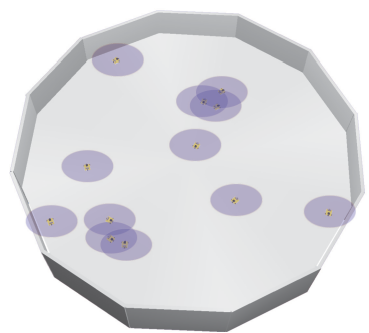
\includegraphics[width=6cm]{cockroachaggsim.png}
\caption{A simulation of the aggregation experiment using robots with communication ranges shown as blue circles surrounding each agent.}\label{fig:roachaggmodel}
\end{subfigure}
\caption{}
\end{figure}

In~\cite{Jeanson2005}, Jeanson et al. showed that a species of cockroach, \emph{Blattella germanica}, exhibited clustering mechanics to form groups using only local information and without knowledge of the global structure of the environment or group sizes. An agent based, biological model is developed and described in the above paper where simple action rules are extrapolated from watching real cockroach aggregation behavior in a closed environment under different lighting conditions.

\begin{figure}[!htb]
\centering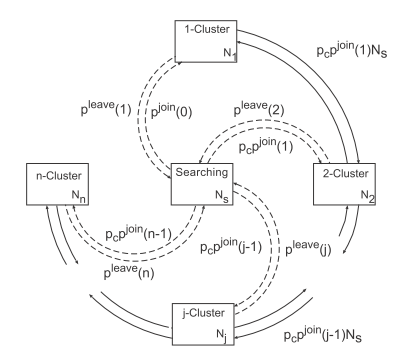
\includegraphics[width=.5\textwidth]{aggfsm.png}
\caption{The PFSM the describes the robot controller for the aggregation experiment. The probabilities shown are probabilities of leaving a cluster of size $n-1$ to join a cluster of size $n$ and vice-versa, as well as the probability to leave a cluster entirely and go back to searching.}\label{fig:aggfsm}
\end{figure}

The data collected from real cockroach aggregation inspired the development of a robotic model for aggregation, as seen in Figure~\ref{fig:aggfsm}~\cite{Correll2007a}. The probabilities for leaving and joining individual clusters are based exclusively on perceived cluster sizes and the time elapsed since joining a cluster. Global information such as actual cluster sizes are not available to any individual agent. Experiments using miniature \emph{Alice} robots were conducted where the robot controller was developed using observed cockroach behavior in~\cite{Jeanson2005}.

\subsubsection*{Results}
In~\cite{Correll2011} the authors theorize that the size of clusters formed by robots can be controlled simply by adjusting their communication range. Specifically, ``For the system with dynamics found in [\ldots eqns representing the robot controller as seen in Figure~\ref{fig:aggfsm}], the system behavior can change between dispersion and aggregation simply by tuning $p_c$ [encountering probability], as long as the inequalities for $p^{join}(j)$ and $p^{leave}(j)$ [probability to join/leave a cluster, respectively] are satisfied.''

\begin{figure}[!htb]
\centering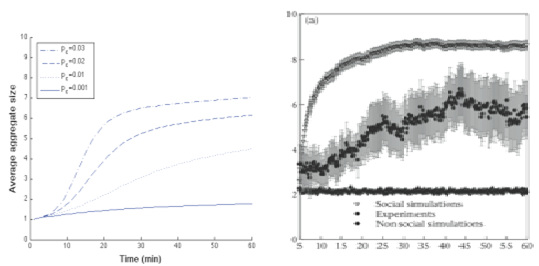
\includegraphics[width=.75\textwidth]{roachRes.png}
\caption{Left: Results of varying communication range and solving macro-model simulation of cockroach aggregation experiment using robotic agents. Right: Results of real cockroach aggregation obtained from experiments and simulation by Jeanson et al. The similarities between both plots are apparent.}\label{fig:roachres}
\end{figure}

Figure~\ref{fig:roachres} shows plots of average cluster sizes observed over time for both, the robotic experiment (left) as well as the experiment involving real cockroaches (right). The robot experiment contains a range of plots for $p_c$ between $0.001$ and $0.03$. We can easily see that the cluster sizes can be made to match the real cockroach experiment just by adjusting the value of encountering probability, which is in turn a function of the communication range of the robots. Conversely, there is the interesting parameter estimation/optimization problem of finding the right $p_c$ to get the desired global behavior (cluster size) from the swarm.

% 5 ============================================================================
\subsection{Collective Inspection Of Regular Structures}

\begin{figure}[!htb]
\centering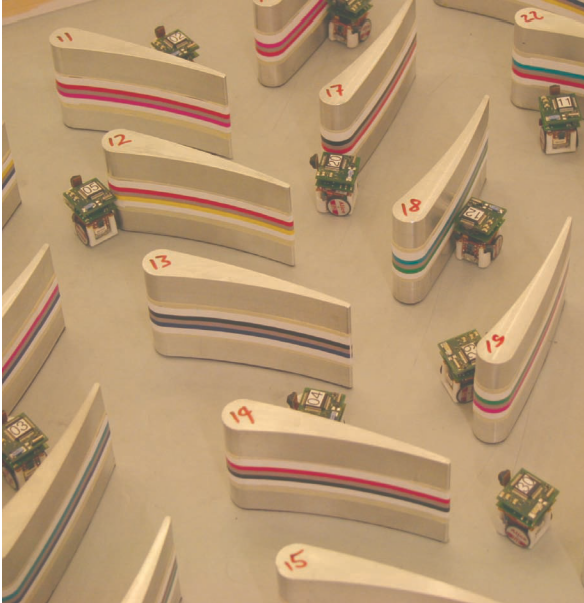
\includegraphics[width=.5\textwidth]{turbexp.png}
\caption{A simplified (unfolded) jet turbine inspection arena with marked blades and Alice robots performing inspection.}\label{fig:turbexp}
\end{figure}

A practical application for swarm systems is proposed by Correll and Martinoli in\cite{Correll2006, Correll2007}. The inspection of airplane jet turbine blades has, so far, been performed manually using borescopes. This procedure is both time and cost intensive and is subject to human error. Automating the task has proven difficult since the shielded, complex, narrow structure of a turbine imposes not only strong miniaturization constraints on the design but also prevents the use of any traditional global positioning and communication system. Furthermore, a limited on-board energy budget might prevent computation of a sophisticated deliberative planning strategy and dramatically narrows the sensor and communication range of our robots.~\cite{Correll2006}

These constraints on the inspection task make it well suited for a miniature robot swarm/multi-agent approach. Since jet turbine blades are regular, repeating structures they provide a good inspection target for robot vision systems.

\subsubsection*{Results}
\begin{figure}[!htb]
\centering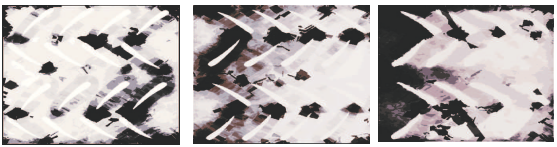
\includegraphics[width=.75\textwidth]{bladeDist.png}
\caption{Distribution of the robots on the arena (dark areas correspond to frequently visited regions). Each experiment lasted 2h with 20 robots. Left: Default setup with the default inspection algorithm. Center: Set-up rotated of 180 degrees. Right: Rotated setup and robots characterized by a random walk behavior.}\label{fig:bladedist}
\end{figure}

Simulation results seen in Figure~\ref{fig:bladedist} show that the probability distribution (agent dispersion and coverage pattern) is non-uniform both, due to the shape of the blades, and border-following algorithm used by robots. It is evident that simply rotating the orientation of the blades results in a different coverage pattern of the arena, by the robots.

\begin{figure}[!htb]
\centering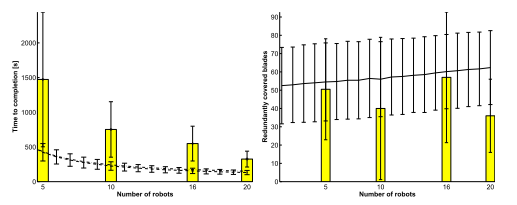
\includegraphics[width=.75\textwidth]{bladeRes.png}
\caption{Comparison of microscopic and macroscopic model predictions (basically superimposed) and experimental results. Experimental results are represented by the median and standard deviation because of long tail distributions while microscopic models by mean and standard deviation. Left: Time to completion (16 blades) vs. team size (1 to 20 robots, 5, 10, 16, 20 robots respectively). Right: Number of blades redundantly covered until inspection completion vs. team size.}\label{fig:bladeres}
\end{figure}

As a result of the inherent spatial nature of the experiment, it is found that both micro-level simulations and macroscopic equations derived for this setup (using the non-spatial methods we have discussed so far) only prove to be qualitatively correct for small robot teams (see Figure~\ref{fig:bladeres}). A more detailed analysis of the model vs. real experiment mismatch is provided by the authors in~\cite{Correll2006, Correll2008a}. We shall see a spatial modeling based approach for the same experiment in the next section.

% 6 ============================================================================
\subsection{Multi-Robot Collaboration Using A Response Threshold Function}

The work by Lerman et. al~\cite{Lerman2001} reinforces results obtained for stick pulling in~\cite{Ijspeert2001, Martinoli1999, Martinoli1999a}. It also extends the original experiment to include the case where more than two robots can be used to pull sticks of variable lengths out of the ground. We build upon this work to introduce a more general algorithm for multi-agent collaboration based on sigmoid response threshold functions, motived from task allocation in insects.

All the collaborative tasks discussed so far are characterized by a binary outcome---success or failure to perform the group task assigned, e.g. pulling a stick out of the ground, or failing to do so. We wish to extend this model to include a more general case of collaboration tasks that involve only approximate number of robots for successful collaboration. Examples of such tasks include collective transport \cite{sugawara2012, Sugawara2013}, pattern recognition \cite{beni1993swarm}, real-time mapping of oil spills \cite{Beni2005}, determining coverage area of forest fires \cite{krishnanand2006glowworm} aerial swarm surveillance, and many others that require a subset of a swarm to coalesce to tackle a task collaboratively. It is important to note that we do not study any particular task in detail but instead, outline a general approach to modeling scenarios with the aforementioned properties. In such cases, so long as we have at least one robot, the task may be accomplished with varying degrees of success. The result is now an accuracy function of the number of robots collaborating on the task, among other environmental factors. 

\begin{figure}[!tp]
\centering\begin{subfigure}{.5\textwidth}
\centering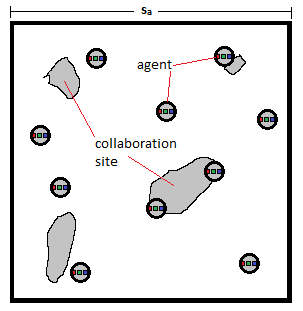
\includegraphics[width=5cm]{setup.png}
\centering\caption{A visual representation of the collaboration experiment being studied. Objects in the image are not to scale.}\label{fig:setup}
\end{subfigure}~
\centering\begin{subfigure}{.5\textwidth}
	\centering\begin{tikzpicture}[->,>=triangle 45,shorten >=2pt,auto,node distance=4cm, semithick,
		state node/.style={rectangle, draw, fill=black!10, minimum height=.8cm, minimum width=1.2cm}]

 	\node[state node] (1) {Search};
 	\node[state node] (2) [right of=1] {Wait};;

	\begin{scope}
		\path	(1) 	edge[bend left] node{$p_{sw}$} (2)
				(2)		edge[bend left] node{$p_{ws}$} (1);
		\end{scope}
		\end{tikzpicture}
\caption{Robot controller used to drive group collaboration. $p_{sw}$ is the probability of going from the search state to the wait state, while $p_{ws}$ is the probability of going to wait to search.}\label{fig:sm}
\end{subfigure}
\end{figure}

We consider a generic collaboration task with $M$ uniformly distributed collaboration sites within a flat arena with side, $s_a$. A swarm of individually simple robots is deployed within the arena, also uniformly and at random as shown in Figure~\ref{fig:setup}. 

The number of robots being used per experiment varies, as we discuss results for a number of different scenarios. The collaboration sites in the arena can be of various sizes and configurations---the only value that is of importance to the model is the total area of all collaboration sites within the arena.

The objective of each agent in the robot swarm is to find a collaboration site in the arena and perform a collective task with other agents at that site. Once this collaboration is complete, the robot detaches itself from its current collaboration site and repeats the search-wait cycle. The precise details of the collective task are not important for the purpose of understanding the coordination mechanism, and we assume collaboration to happen instantaneously for the purpose of the model studied in this paper. The robot controller that describes individual agent behavior for this swarm system is shown in Figure~\ref{fig:sm}.

The population dynamics equations and the threshold function used for the model are described below. The associated PFSM is seen in Figure~\ref{fig:sm}
\begin{equation}
	p_{ws}(\sigma) = \frac{1}{1 + e^{\theta(-\sigma + \tau)}}\label{eq:sigmoid}
\end{equation}
\begin{align}
	N_s'(t) = & N_w(t)p_{ws}(\sigma) - N_s(t)p_{sw}\label{eq:macro1}\\
	N_w(t) = & N_0 - N_s(t)\\
	N_s(0) = & N_0\\
	N_w(0) = & 0\label{eq:macro4}
\end{align}
In equation~\eqref{eq:sigmoid} control parameter $\theta$ controls the slope of the sigmoid function, while $\tau$ controls its offset along the $\sigma$ axis, as seen in Figure~\ref{fig:sig}. The input-$\sigma$ to the probability function $p_{ws}$ within an individual robot controller is the number of agents currently at the same collaboration site as the robot. But group sizes at collaboration sites are not tracked in the macro-model and so we re-define $\sigma$ as the average group size at time $t$, i.e. $\sigma(t) = N_w(t)/M$. Within the context of the swarming task, $\tau$ is the desired collaboration threshold value, while $\theta$ controls the variance or degree of flexibility we want the group sizes to have.

\begin{figure}[!htb]
\centering\begin{subfigure}{.5\textwidth}
\centering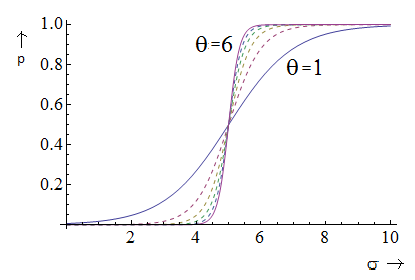
\includegraphics[width=6.5cm]{sigmoid1.png}
\caption{Increasing $\theta$ in the sigmoid function increases it's slope at the point $\sigma^* = \tau$, $p_{ws}(\sigma^*) = 0.5$.}
\end{subfigure}~
\centering\begin{subfigure}{.5\textwidth}
\centering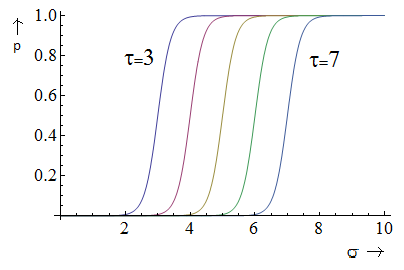
\includegraphics[width=6.5cm]{sigmoid2.png}
\caption{Changing the $\tau$ parameter in the sigmoid function, offsets the curve along the $\sigma$ axis.}
\end{subfigure}
\caption{}\label{fig:sig}
\end{figure}

\subsubsection*{Results}
\begin{figure*}[!ht]
\centering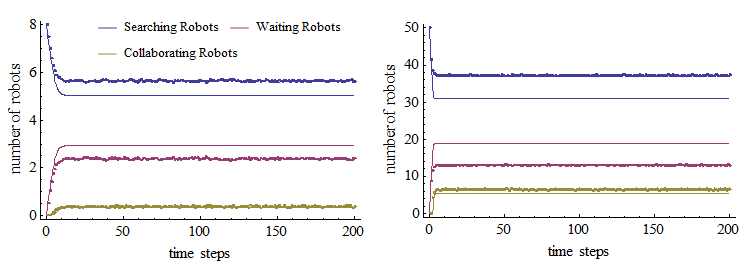
\includegraphics[width=\textwidth]{macmic.png}
\caption{Macro-level numerical solutions and micro-level Gillespie simulation data plots for the proposed collaboration model. Left: $N_0 = 8$, $M = 2$, $\theta = 4$, and $\tau = 2$. Right: $N_0 = 50$, $M = 5$, $\theta = 5$, and $\tau = 4$. Data plotted for 200 seconds of simulation time and 100 runs each.}\label{fig:macmic}
\end{figure*}

We numerically solve the rate equations with the given initial condition that all robots start off in the search state(\eqref{eq:macro1} to \eqref{eq:macro4}), for $N_s(t)$, $N_w(t)$ and $R_c(t)$, from $t = [0, 200]$. Here, $R_c(t)$ is not a state variable of the robot controller but is an aggregated value that measures the collaboration rate of the system at each time step and is mathematically described by
\begin{equation}
R_c(t) = N_w(t)p_{ws}(\sigma)
\end{equation}
i.e., the number of robots going from the wait state to the search state at time $t$.

Numerical solutions for the rate equation are shown in Figure~\ref{fig:macmic}, along with data from the microscopic simulation for the same quantities. The two plots show that the system approaches a steady state distribution of agents for each of the two states. We perform the macro-level solution and the micro-level experiments with two sets of system parameters. The left plot in Figure~\ref{fig:macmic} shows results from experiments conducted using 8 robots, 2 collaboration sites, expected group sizes $\tau = 2$, and the sigmoid slope parameter $\theta = 4$. The right plot in Figure~\ref{fig:macmic} shows results using $N_0$ = 100 robots, $M = 5$ collaboration sites, $\tau = 5$ expected group size, and $\theta = 4$. The data points for the microscopic model are averaged over a hundred runs per point.


\begin{figure*}[!ht]
\centering\begin{subfigure}{7.5cm}
\centering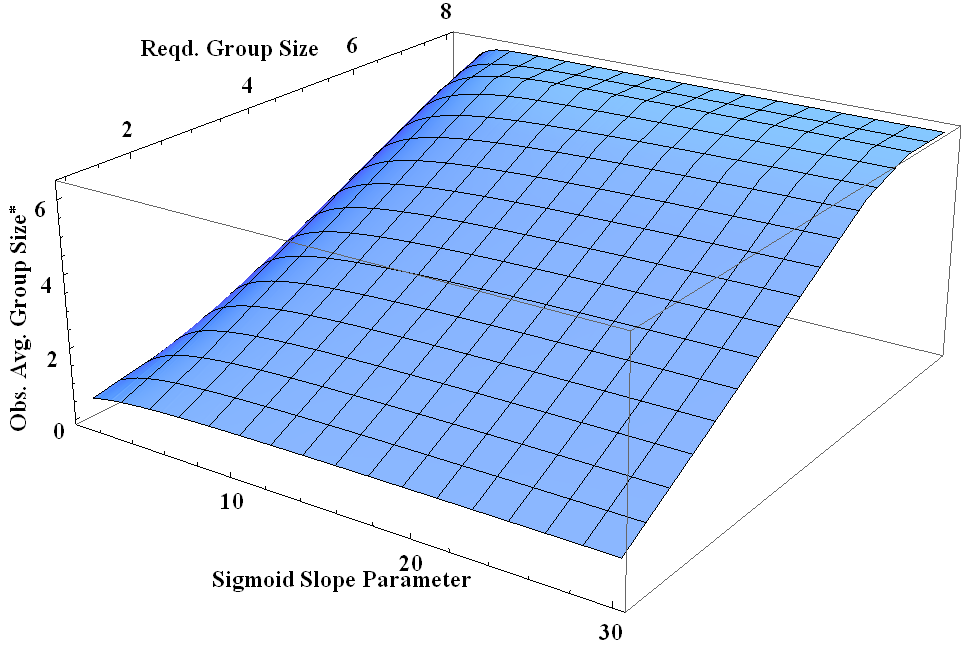
\includegraphics[width=7.5cm]{macroSweepM1.png}
\caption{$M = 1$}\label{}
\end{subfigure}~
\centering\begin{subfigure}{7.5cm}
\centering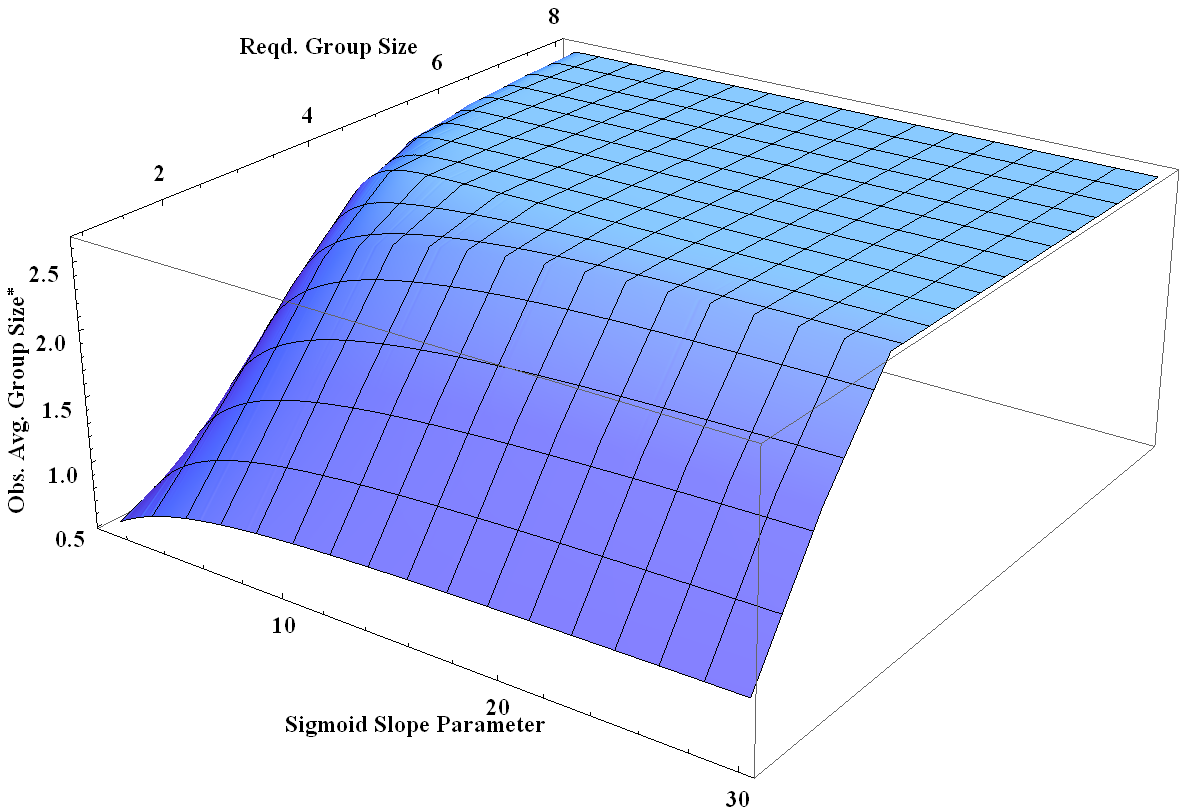
\includegraphics[width=7.5cm]{macroSweepM3.png}
\caption{$M = 3$}\label{}
\end{subfigure}~
\caption{Numerical solutions for the rate equations~\eqref{eq:macro1} to \eqref{eq:macro4} with $N_0 = 8$ and $t = [0, 200]s$ as we sweep the sigmoid control parameters, $\theta$ and $\tau$.}\label{fig:sweeps}
\end{figure*}

Figure~\ref{fig:sweeps} showcases the macro-level behavior of the swarm system when we sweep across $\theta$ and $\tau$, numerically solving the rate equations. As the slope of the sigmoid at $\sigma^*$ gets higher, we expect to see system behavior and average group sizes resembling that as if a step function was used instead of the sigmoid probability function, i.e. for $\theta \gg 1$, 
\begin{equation*}
p_{ws}(\sigma) \approx \Theta(\sigma) = \left\{
\begin{array}{rl}
1 & : \sigma \geq \tau\\
0 & : \text{o/w}
\end{array}\right.
\end{equation*}
The sloped portion of the graphs reinforces this assertion that setting higher values for $\theta$ does indeed result in average observed group sizes being close to the requested collaboration threshold using the $\tau$ parameter. As the slope parameter, $\theta$, is reduced, we see a marked drop in the correspondence between observed vs. requested group sizes. We also see that increasing $\theta$ past a certain point results in no major observed vs. requested group size shift.

\begin{figure}[!tp]
\centering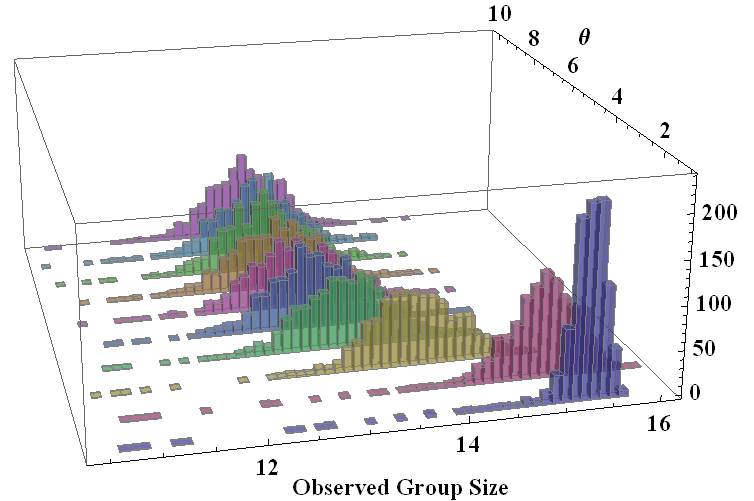
\includegraphics[width=7cm]{distsweep.png}
\caption{Relative distribution of robot group sizes as $\theta$ is varied, while keeping all other parameters constant.}\label{fig:var}
\end{figure}

Finally, we are interested in studying the distribution of group sizes during the course of the experiment, as the sigmoid slope parameter is varied. Figure ~\ref{fig:var} shows a 3D histogram of observed group sizes for increasing $\theta$ values, from 1 to 10, over 200 seconds of Gillespie simulation time, using a 100 robots, 5 collaboration sites, and a threshold value of 20. All values a averaged over 100 simulation runs.

\end{document}